\section*{\textsc{библиография}}
\addcontentsline{toc}{section}{\textsc{\textbf{библиография}}}
\label{sec:10}

\subsection*{А.\=,Эйнштейна. <<О специальной и всеобщей теории относительности>>}
\addcontentsline{toc}{subsection}{11. А.\=,Тимирязев\---А.\=,Эйнштейна. <<О специальной и всеобщей теории относительности>>}
\label{subsec:10.1}

А.\=,Эйнштейна. О специальной и всеобщей теории относительности (общедоступное изложение) 12\-/е издание (51\--55 тысяч) 91\=,стр. 1921\=,г. Издание Фивега. Ueber die Spezielle und die Allgemeine Relativit\"{a}tstheorie (Gemeinvelrst\"{a}ndlich) von A.\=,Einstein Zw\"{o}ltte Auflage (51\--55 Tausend) Vieweg 1921\=,г. Имеются три перевода на русский язык., один издан в Берлине, другой в Петербурге \footnote{Перевод с V нем. изд. С.\=,Вавилова, п. ред. А.\=,Афанасьева, издание <<Научное книгоиздательство>>. ПБ. 1921\=,г.}) и третий на днях выпускается Госиздатом.

Теория относительности знаменитого физика Альберта Эйнштейна привлекает к себе внимание настолько широких кругов обитателей земного шара, что без всякого преувеличения можно сказать: никогда ещё ни одна научная теорема не находила столь живого отклика среди людей, стоящих далеко от науки и мало обыкновенно интересующихся её текущими задачами. Этой теорией интересуются люди самых противоположных взглядов\---самых противоположных складов мысли. Одни считают её самым блестящим проявлением новой, свежей научной мысли, проводимой убежденным революционером в науке, в последние годы после войны открыто ставшим на сторону борющегося рабочего класса. Другие приветствуют эту теорию также как великую революцию в науке и главное её достоинство видят в том, что она наносит <<смертельный удар>>\dots\ материализму! Т.\=,е. будто бы подрывает в корне основы величайшего из революционных учений, связанных с именами Маркса и Энгельса.

Последняя категория <<друзей революции>> в науке в настоящее время встречается в большом изобилии на всём земном шаре. Люди этого толка, ненавидя революцию в общественной жизни, восторгаются ею в науке потому, что революция в науке для них равносильна уничтожению науки и восстановлению авторитета религии и находящихся на её службе различных течений идеалистической философии.

Разберём, насколько это возможно, в краткой заметке, на чём основывается эта бесплодная попытка повести атаку на самые основы материализма. Прежде всего, однако, в чём же состоит принцип Эйнштейна? В основе его теории находится следующее положение:

\emph{Законы всех явлений природы не зависят от состояния движения изучающего их наблюдателя.} На первый взгляд в этом утверждении нет ничего удивительного и непонятного. Представьте себе, что Вы сидите в вагоне равномерно идущего поезда и Вы роняете из рук какой-нибудь предмет на пол вагона: он упадет совершенно также и попадет в то же самое место пола, как\-/будто бы поезд и не двигался. Вы можете перекидываться мячиком с сидящим против Вас вашим соседом; мяч будет перелетать в ту и другую сторону так, как\-/будто поезд был неподвижен. Мы часто даже не замечаем движения поезда, если он идет без толчков\---равномерно. Вспомните, например, когда на станции перед окном вагона, в котором Вы сидите, стоит вагон другого встречного поезда. Вы слышите свисток, замечаете движение, но не можете сразу решить, который из двух поездов пошел? Таким образом участие наблюдателя в равномерном и прямолинейном движении не влияет сколько\-/нибудь заметным образом на характер явлений, которые он наблюдает и изучает.

Дело становится гораздо труднее, если мы попытаемся распространить положение Эйнштейна на более сложные явления, как например, на измерение скорости света. Пусть, например, на платформе, расположенной вдоль железнодорожного пути, измеряют скорость света. Луч вышел из А и через некоторый,
\begin{figure}[htp]
 \centering
 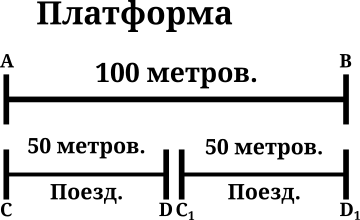
\includegraphics{2.png}
 \label{fig:1}
\end{figure}
очень малый промежуток времени приходит в В, пройдя всю длину платформы в 100 метров. Чтобы найти скорость света надо знать, сколько времени потребовалось свету, чтобы пройти эти сто метров. Пусть теперь скорость света измеряют с поезда, который за время, в течение которого свет прошел из конца в конец платформы, передвинулся из $ CD $ в $ C_{1}D_{1} $. Когда луч света выходил из А, против А было последнее окно последнего вагона поезда. Когда луч света будет у другого конца платформы, там будет находиться переднее окно первого вагона (считая от паровоза). Для наблюдателя в поезде свет прошел всю длину поезда, которая на нашем чертеже в два раза меньше длины платформы. Таким образом, рассчитывая скорость света \emph{для себя,} он найдёт её в два раза меньшей, чем наблюдатель, стоящий на платформе. Для одного свет пройдет, считая вдоль поезда,50 метров, для другого \emph{за то же время}\---100 метров. Как же быть теперь с принципом Эйнштейна, требующим, чтобы скорость света как и всякое другое явление в природе не зависело от движения наблюдателя? Выход один: \emph{надо допустить, что все часы в поезде} и вообще все, чем можно измерить время, \emph{идет медленнее,} т.\=,е. само время течет медленнее для того, кто движется. Этим мы спасаем принцип Эйнштейна: действительно, раз пройденный светом вдоль поезда путь меньше, но зато и промежуток времени, отмеренный медленно идущими часами также стал меньше, тогда скорость может получиться та же самая, как и для наблюдателя на платформе! \footnote{В действительности осуществить измерение скорости света в той форме, как это у нас описано, невозможно. Это опыт воображаемый, он приведён только для того, чтобы выяснить более наглядно ход мыслей Эйнштейна. В теории относительности так поступают на каждом шагу. Вся книжка Эйнштейна переполнена описаниями воображаемых опытов подобных изложенному.}). Более обстоятельный и строгий разбор этого явления показывает, что для оправдания основного положения Эйнштейна необходимо помимо допущения об изменившемся ходе времени допустить ещё, что в зависимости от скорости движения все предметы сжимаются по направлению движения, так что движущийся поезд должен быть немного короче неподвижного, \emph{правда, это укорачивание равно, как и замедление хода времени, согласно теории должно быть ничтожно малым даже для самых быстро движущихся аэропланов;} И самое главное мы никогда не в состоянии этого проверить, потому что в движущемся вагоне и аэроплане \emph{все часы изменят свой ход} и все аршины и метры укоротятся. Таким образом, эта теория очень хорошо застрахована от опытной проверки! Рассмотренная нами сейчас часть теории Эйнштейна, называемая <<специальной теорией относительности>>, занимает почти две трети книжки Эйнштейна, Эта часть книги читается легко. В 1916 году Эйнштейн опубликовал свою <<Всеобщую теорию относительности>>, где им сделана попытка распространить основное положение его теории на любой вид движения, в том числе и вращательное. Для этого приходится сделать еще один шаг, приходится отказаться от основ нашей геометрии, которую мы изучаем в наших школах и которая ведёт своё начало от великого греческого геометра Эвклида. Этой геометрией мы ежеминутно пользуемся в наших практических расчетах и постройках вплоть до самых сложных технических сооружений и до сих пор никогда не имели случая раскаиваться. Чтобы отстоять своё положение о неизменности законов природы от состояния движения, изучающего их наблюдателя, Эйнштейну приходится заменить знакомую нам геометрию Эвклида одним из тех воображаемых построений, какие были созданы позднейшими геометрами, в том числе и Н.\=,Лобачевским, и которые имеют большой теоретический интерес. Эйнштейн этим воображаемым построениям придаёт реальный смысл и опять так же, как и в специальной теории, указывает, что отступления от эвклидовой геометрии должны быть ничтожно малы, но по его теории они должны быть!

Есть ли, однако, необходимость, вынуждающая нас безоговорочно согласиться с этими допущениями, с которыми здоровый рассудок не может, по крайней мере, сразу примириться?

На это мы можем решительно ответить: нет! Все выводы из теории Эйнштейна, согласующиеся с действительностью, могут быть получены и часто получаются гораздо более простым способом при помощи теорий, не заключающих в себе решительно ничего непонятного\--- ничего сколько\-/нибудь похожего на те требования, какие предъявляются теорией Эйнштейна.

В этом отношении надо отдать полную справедливость Эйнштейну, в своей книжке он определённо указывает, что всё, что вытекает из его теории, может быть получено независимым от его теории путем; он видит в этом особое достоинство своей теории, дающей то же самое, что и все остальные, но зато обладающей философским единством, которое свойственно только ей одной.

Вторая часть книги, посвященная всеобщему принципу относительности, изложена хуже: многое приходится читателю принимать на веру.

На чём же строят свои нападки на материализм сторонники и последователи Эйнштейна? (Надо заметить, что сам Эйнштейн, хотя и высказывает иногда мысли, идущие в разрез с философией материализма, но никакого активного похода против основ материализма не ведёт).

Прежде всего, если для каждого наблюдателя в зависимости от его движения время идет определенным ходом, отличающимся от хода времени для других наблюдателей, двигающихся иначе, и если в зависимости от движения изменяются размеры предметов, то значит объективно вне нас существующего пространства и времени нет! Но ведь изменившийся ход часов, который мы не можем проверить, мы должны были придумать для того, чтобы навязать природе основное положение Эйнштейна и чтобы не впасть в противоречие с фактами!

Далее для той же цели мы должны подобрать определенное искажение реальной геометрии и приписать ей реальное существование. Из этого делают вывод: любая геометрия эвклидова или неэвклидова есть чистый продукт разума, независящий от опыта. Все эти системы геометрии существовали в сознании и вот из них Эйнштейн подобрал такую, которая теоретически ближе всего подходит к действительности, и геометрия Эвклида ничем не отличается от остальных.

Но этот довод устраняется крайне просто: \emph{все воображаемые системы геометрии в отличие от эвклидовой возникли после неё, как попытки построить системы, отличные от того, что есть:} они не могли бы и возникнуть, не будь раньше нам известна геометрия Эвклида, которая подтверждается буквально на каждом шагу в нашй практической деятельности, подобно тому, как всякая фантазия\---всякая сказка не могла бы возникнуть, если бы мы не знали той были, той действительности, которой она противополагается.

Наконец из того, что для оправдания принципа Эйнштейна о независимости законов природы от движения наблюдателя, человек подбирает определенным образом ход часов и ту или другую воображаемую геометрию объявляет реальной и заменяет ею практически нам необходимую евклидову, делается вывод, что не сознание складывается под влиянием воздействия независимо от нас существующего мира, а, что наоборот, сознание предписывает этой реальной действительности свои законы!

Ошибки здесь в том, что, приписав природе произвольное допущение Эйнштейна, мы потом должны подыскивать такие новые допущение, который не дали бы нам возможности разойтись с фактами. Забыв при этом, что мы это вынуждены делать потому, что мы сделали произвольно первый шаг. И вот об этом своеобразном процессе подлаживания под действительность: шаг назад и шаг вперед, громогласно объявляют: сознание диктует бытию свои законы!

Отчего же в здоровой науке, где, как указывает тов.\=,В.\=,Ленин, ученый <<стихийно>> становится материалистом возникают такие нездоровые течения? Ответ может быть один: вопросы, связанные с теорией относительности, касаются таких областей, где мы при наших технических средствах ещё не можем решить дело лабораторными опытами. А там, где ученый\=/естествоиспытатель лишается своей единственной верной опоры, ум его очень легко может свихнуться.

Необходимо, однако, оговориться: в теории Эйнштейна, помимо теории относительности, много весьма ценного. Его попытка обосновать теорию всемирного тяготения имеет громадный интерес, но она непосредственно не связана с принципом относительности.

Во всяком случае книжка Эйнштейна представляет лучшее изложение теории относительности; она называется общедоступной, но читать её может лишь тот, кто усвоил основы алгебры и геометрии, хотя бы в том объеме, в каком эти отрасли знания преподаются на рабочих факультетах.

\begin{flushright}
 \textbf{А.\=,Тимирязев.}\hspace*{2em}
\end{flushright}

\subsection*{К.\=,Маркс и Ф.\=,Энгельс. Собрание сочинений, том III, Гос. Изд. 1921\=,г., стр.\=,520.}
\addcontentsline{toc}{subsection}{12. В.\=,Р.\---К.\=,Маркс и Ф.\=,Энгельс. Собрание сочинений, том III}
\label{subsec:10.2}

Судьба собрания сочинений Маркса н Энгельса весьма поучительна. Книгоиздательство <<Коммунист>> ещё в 1918 году объявило об организации специальной редакции для издания сочинений Маркса и Энгельса, при чём тогда же было опубликовано примерное содержание каждого тома, каковых предполагалось выпустить <<до 28 томов по 26\--30 листов большого формата>>. Программа была самая широкая. <<В это юбилейное издание войдут как все работы, появившиеся до сих пор в Германии и Англии отдельными изданиями, так и работы рассеянные по разным периодическим изданиям>>.

Но вот прошло уже четыре года, а из этой программы выполнена самая незначительная часть изданы два тома <<Капитала>> (собр. соч., т.\=,IV и V) и вот перед нами лежит третий том собрания сочинений\---собрание исторических работ.

Нет бумаги! а на ведомственную макулатуру бумага есть? Ведь, если бы хоть на одну четверть сократить издание продуктов <<чиновничьего усердия>>, то мы бы имели возможность издавать ни одного Маркса, но и всех классиков социализма и коммунизма!

Вот и те тома, которые лежат перед нами. Как они изданы? Из рук вон плохо: бумага циллюлозная\---полугазетная (в IV и V томах) и газетная (в третьем томе), брошюровка, отвратительная, без всяких подшивок\---как развернёшь, так книга вся и расползает, печать местами совершенно слепая\---словом, как нарочно, сделано так, что с самого начала вызывает в читателе негодование.

Государственному Издательству нужно энергично взяться за издание, столь необходимое нашей рабочей интеллигенции.

Кстати несколько слов о редакции: в числе имён сотрудников издания вы не встретите Д.\=,Б.\=,Рязанова; это очень жаль, такой прекрасный знаток Маркса и Энгельса, как Д.\=,Б.\=,Рязанов, мог бы дать очень многое такого, чего вряд ли смогут дать перечисленные в списке авторы: вследствие чрезмерной занятости одних и сравнительно малой компетентности других.

А теперь несколько слов о третьем томе.

Как мы уже отметили выше, внешность крайне неряшлива: одна желтоватая обложка из обёрточной бумаги что стоит! Но кроме чисто\=/технических недостатков имеется и ряд весьма заметных внутренних дефектов, на которые мы вкратце и хотели бы указать. Этот том составлен из пяти следующих статей:
\begin{enumerate}
 \item К.\=,Маркс\---<<Борьба классов во Франции 1848\--1850\=,гг.>>
 \item К.\=,Маркс\---<<\glqqВосемнадцатое\grqq, брошюра Луи Бонапарта>>.
 \item Ф.\=,Энгельс\---<<Революция и контр\=/революция в Германии>>.
 \item К.\=,Маркс\---<<Перед судом присяжных в Кёльне>>.
 \item К.\=,Маркс\---<<Разоблачения о Кёльнском процессе коммунистов>>.
\end{enumerate}

С первого же взгляда бросается в глаза отсутствие почему\-/то <<собрания \emph{исторических} работ Маркса и Энгельса>>, <<Гражданской войны во Франции>>. Хотя по проспекту 1918 года она должна была быть включена.

Отсутствуют совершенно примечания, не отмечены ни годы появления статей, ни обстоятельства, вызвавшие их: при иных статьях имеются предисловия авторов, где в общих чертах дается ряд сведений, статью Ф.\=,Энгельса\---<<Революция и контр\=/революция в Германии>> снабдил предисловием редактор\---тов.\=,И.\=,Степанов. Но всё это совсем недостаточно. Затем\---совершенно отсутствует регистр\-/указатель, хотя бы какой\-/нибудь. В Западной Европе даже самая на наш взгляд обыкновенная книга снабжается указателями, а мы выпускаем К.\=,Маркса и Энгельса без намека на указатель!

Это очень трудно составить\---конечно трудно, что и говорить; но ведь нельзя же из\-/за кое\-/каких затруднений так безбожно портить и обесценивать книгу. В том виде, в каком эти статьи предподнесены читателю, в третьем томе значительно затрудняется пользование ими. Нужно всемерно ускорить выпуск собрания сочинений Маркса и Энгельса, Госиздату следует требовать от своих техников и спецов (которые и в наши дни не разучились хорошо издавать книги) внимательного отношения к этому изданию ведь вся рабочая интеллигенция ждет не дождется выхода остальных томов!

\begin{flushright}
 \textbf{В.\=,Р.}\hspace*{2em}
\end{flushright}

\subsection*{Письма Г.\=,В.\=,Плеханова к П.\=,Л.\=,Лаврову}
\addcontentsline{toc}{subsection}{13. В.\=,Румий\---Письма Г.\=,В.\=,Плеханова к П.\=,Л.\=,Лаврову}
\label{subsec:10.3}

(<<Дела и дни>>\---исторический журнал, 1921, книга II, печ. Гос. Изд.).

Во втором номере исторического журнала <<Дела и Дни>> появились двадцать два письма Г.\=,В.\=,Плеханова к П.\=,Л.\=,Лаврову. Они так характерны для Плеханова, что невольно приковывают к себе внимание читателя.

Они все относятся к периоду 1880\--1883, т.\=,е. к тому весьма интересному периоду, когда группа <<Черный Передел>> во главе с Г.\=,В. проделывала эволюцию от народничества к марксизму.

Разумеется эти письма не достаточны, чтобы на их основании иметь детальное исчерпывающее представление о жизни и идейном развитии Плеханова и его товарищей в эту эпоху. Однако в приведенных письмах масса весьма ценных указаний и материала.

Здесь Плеханов\--- непримиримый и непреклонный \--- когда дело касается теории\--- выступает перед вами в первом же из опубликованных писем.

К объявлению <<Об издании Русской Социально\=/Революционной Библиотеки>>, написанном Плехановым, Пащенко прибавил несколько слов о малороссийской литературе. В этом прибавлении Пащенко одобрительно отзывался о брошюре Липского, <<Про те, як наша землья стала не наша>>; в этой брошюре автор её развивает мнение, будто <<украинские крестьяне чувствовали бы себя лучше если бы паны на Украине были не польские и не русские, а свои же украинские>>. Это украинофильское мнение вопиюще противоречит основным положениям социализма. <<И поскольку оно противоречит социализму, постольку эта и ей подобные брошюры не могут называться научными. \emph{Там, где нет социализма\--- нет науки. Вот почему там, где есть хоть одна строка, написанная мною, не может быть похвалы гг. украинцам}>>. Он настаивает, чтобы в случае несогласия парижских товарищей выбросить эту <<похвалу>>\---предали бы сожжению им написанное <<объявление>>. \emph{И три} раза в одном письме протестует он против того, что выдают <<похвальный лист>> украинофилам <<за то, что они морочат голову украинского мужика>>. Это, повторяем, крайне характерно для Плеханова.

Эта же суровая последовательность и настойчивость прорываются в этих письмах не раз: объясняя Лаврову причины нежелания принять на себя звание редактора <<Вестника Народной Воли>> он между другими выставляет ту, что между ним и С.\=,Кравчинским серъёзная разница в воззрениях: <<Он что\-/то в роде прудониста, я\---\emph{не понимаю} Прудона; \emph{характеры} наши \emph{тоже несовсем сходны}: он человек, относящийся в высшей степени терпимо ко всем оттенкам социалистической мысли, \emph{я готов создать из \glqqКапитала\grqq\ Прокрустово ложе для всех сотруников \glqqВестн. Народн. Воли\grqq>>.} Уже теперь, в начале 1882 года, Плеханов\---совершенно законченный тип революционного <<характера>>\---ортодокса до <<фанатизма>> и непримиримого до конца\---каким мы знали его до его смерти, по крайней мере в области теории.

Как работал этот непреклонный <<фанатик>>?

В наши дни жизнь развертывается с такой головоокружительной быстротой и всё кругом нас творится и рушится с такой стремительной силой, что почти безотчётно этот процесс переносится в область умственного и научного труда.

Писать сегодня статью? читать лекцию? да ведь это же дело двух минут!

Потому\-/то теперь трудно разыскать глубоких и садержательных статей, слышать хорошую речь.

Не так работал Плеханов. Он пишет статью после основательного изучения вопроса. <<Такова моя несчастная привычка, к каждой статье готовиться, как\-/будто я собираюсь писать диссертацию>>. После первой статьи о Родбертусе ему Михайловский предложил написать вторую статью о нём же. Он собирает все его сочинения, которых много <<хотя и не волюминозны>>. Для этого он пишет П.\=,Лаврову, собирается ехать в Берн, при всей своей бедности решается приобрести их у берлинских книгопродавцов в случае, если их не найдёт в Берне: <<не знаю удастся ли\---достать; а без остальных соченений я писать о нём не стану>>. Он думает рыться в газетах того времени, что бы найти материал о его деятельности как министра в 1848\--50\=,гг.

Он и на самом деле работал к своим статьям так, как не работает для своей диссертации иной доцент. <<Целые дни сижу я за своей статьёй>>\--- не всякому пишущему <<статьи>> знакомо такое настойчивое трудолюбие.

До сих пор не имеется достаточно материалов для определении процесса \{\dots \} и развития марксистских идей в России до момента опубликования брошюры Плеханова <<Социализм и политическая борьба>>. Обычно момент организации <<Гр. Осв. Тр.>> (1883\=,г.) берется за начало. Но разве Плеханов уже не был марксистом, когда готовился сделать из <<Капитала>> Прокрустово ложе для сотрудников <<Вести. Нар. Воли>>? А это было в \emph{начале 1882 года.}

Письма эти крайне ценны, хотя и недостаточны. Они лишь чуть чуть углубляют наш взор, не давая по этому вопросу исчерпывающих материалов. Очень интересно письмо под номером 15 (лето 1883\=,г.), где Плеханов подвергает критике <<объявление об издании журнала \glqqВести. Нар. Воли\grqq>> Тут впервые он формулирует идею <<народного государства \emph{с прямым народным законодательством}>>, идею, впоследствии (1884\=,г.) повторенную в <<Проекте программы Гр. Осв. Тр.>>.

Яснее всего в этих письмах выступает его крайне стесненное, невероятное бедное материальное положение. Как ни был сдержан Плеханов, как он ни пренебрегал нуждой и не трудился, всё же без помощи друзей, особенно Лаврова, обходиться не мог. Получив за статью 500~руб., <<я должен уплатить свои долги, которых на мне больше, чем на русском государственном казначействе. Уплачивая же долги, я должен иметь в виду степень потребности в деньгах со стороны моих кредиторов, \emph{так как всех зараз уплатить мне невозможно}>>.

В другом письме от 6 февраля 1882 года он пишет Лаврову:

<<Извините, что пишу на carte postale\--- не имею \emph{покупательной силы в данную минуту}>> (курсив мой).

Покупательной силы на одно закрытое письмо!

П.\=,Л.\=,Лавров в это время много помогал Плеханову: ссуживал деньги, снабжал его материалами для работ, давал литературные работы и рекомендации. <<Благодаря Вашей поддержке, я, быть может, получу возможность работать и развиваться, не имея в перспективе \emph{голодной смерти или задолжения без надежды уплаты}>>, пишет он, <<Вы (Лавров), Маркс и Чернышевский были любимейшими моими авторами, воспитывавшими и развивавшими мой ум во всех отношениях>>\--- тут несомненно следует быть весьма осторожным, ибо, громадной степени это утверждение\---плод большой вежливости Плеханова. То что Чернышевский был любимейшим писателем его и оказал большое влияние на развитие его\--- несомненно. Но на счет П.\=,Лаврова\--- это можно принять весьма условно. Нам кажется, Плеханов был гораздо искренней впоследствии, когда оценивал ларвизм как <<эклектизм на идеалистической подкладке>> и находил, что <<те из наших революционеров, которые основательно прошли эту школу и сроднились с употреблявшимся в ней методом мышления \emph{навсегда лишились способности понять учение Маркса}>>. (Пред, к Туну\--- Изд. Пер. Сов. 1818\=,г., стр.\=,29).

Из этого беглого обзора читатель видит как много содержат в себе эти письма.

Нам кажется следовало бы поспешить с опубликованием писем Плеханова всем, у кого они имеются\--- они прольют на многие вопросы истории марксизма и нашей партии яркий свет и воссоздадут прекрасный образ непримиримого Г.\=,В.\=,Плеханова.

Еще несколько замечаний о датах писем. Некоторые из них без дат и Л.\=,Дейч восстанавливая их по компетентному указанию Д.\=,Б.\=,Рязанова сделал ряд ошибок. В <<Собрании сочинений>>, куда они войдут, даты нужно установить более точные.

\begin{flushright}
 \textbf{В.\=,Румий.}\hspace*{2em}
\end{flushright}

\subsection*{Гибриель Девиль <<Научный Социализм>>. Перевод Мещерякова. Москва. 1919\=,г.}
\addcontentsline{toc}{subsection}{14. Б.\=,Ш.\---Гибриель Девиль <<Научный Социализм>>. Перевод Мещерякова}
\label{subsec:10.4}

Новое издание очерка Девиля, написанного еще в 1883 году, может вызвать некоторые недоумения. Однако мысли Девиля за 40 лет не потеряли своего интереса. Девиль говорит, что работа была предпринята <<по любезному приглашению и при дружеском одобрении К.\=,Маркса>>. И действительно очерк проникнут насквозь революционным духом Маркса.

Тактика рабочего класса в борьбе с капиталистическим обществом, первые шаги его в новом, неизбежно приближающемся, уже недалеком, обществе\--- вот что занимает Девиля. В отвлечённых теоретических вопросах заметно сказывается его основной недостаток\---некоторая инертность диалектики. <<Мысль есть \emph{только} интелектуальное \emph{отражение} реального движения вещей>>. <<Весь ход человеческого прогресса был результатом применения насилия>>. Так схематизирует недостаточно гибкая мысль Девиля диалектику жизни. Он не дооценивает значение государственного капитализма, который для него, <<не является результатом естественного хода вещей>>. Поэтому же терпит он неудачу в попытке применить законы Дарвина к человеческому обществу.

Насилие, революция, разрушение буржуазного государства, диктатура\--- здесь полная чёткость и уверенность у Девиля. Партия, хотя бы и меньшинство,\---вождь класса на этом пути.

Самая жестокая, беспощадная критика парламентаризма, реформизма, буржуазных свобод. Блестяще скрывает он реакционность лозунга буржуазной свободы личности для пролетария.

С прозорливостью пишет он о первых победных шагах рабочего класса: <<Мы стремимся не к установлению одним ударом общественного строя, план которого изобразили, а к замене капиталистического строя таким, элементы которого развиваются с каждым днём в недрах существующего. Но этот переворот обусловливается предварительным захватом политической власти>>. Крестьянство <<рабочая партия может привлечь к коммунистическому строю только терпеливо выжидая, чтобы ход вещей совершил эту неизбежную экспроприацию>>. <<Следовательно по отношению к крестьянству будут прибегать не к насилию, а к убеждению>>. Везде, написанное за десяток лет до Эрфутской программы, звучит борьбой современности. Дух революционного марксизма, проникающий книгу, даёт не только правильную схему марксовского социализма, но и возможность более вдумчивому читателю сравнять свой опыт с предвидениями молодой марксистской мысли.

\begin{flushright}
 \textbf{Б.\=,Ш.}\hspace*{2em}
\end{flushright}

\subsection*{Франц Меринг. Исторический материализм. Издательство ВЦИК Советов Москва, 1918\=,г.}
\addcontentsline{toc}{subsection}{15. Б.\=,Пинсон\---Франц Меринг. Исторический материализм}
\label{subsec:10.5}

Брошюра Ф.\=,Меринга <<Исторический материализм>> представляет собой крайне удачную попытку в кратком, сжатом, хотя и не совсем популярном виде, передать сущность материалистического понимания истории, как философской системы, в основу которой положен диалектический метод Маркса и Энгельса.

В самом начале вскрывается классово\=/враждебное отношение буржуазии, её идеологов и казённых учёных к историческому материализму, и вместе с тем справедливо отмечается, что до последнего времени, несмотря на все потуги, буржуазная критика не сумела с достаточной серьезностью подойти к этой сравнительно молодой философской школе.

Сам исторический материализм является продуктом исторического развития; только на известном этапе капиталистического развития можно было найти и точно установить <<двигательные причины истории>>.

Этим этапом, как указывает Фридрих Энгельс, явился период развития промышленного капитализма, когда на политической арене рядом с конкурирующими между собой и борющимися за политическое влияние двумя классами\--- крупными землевладельцами и буржуазией\---явился новый класс или третья сила, вызванная к жизни самим капитализмом\---пролетариат.

Он обрушивается на дуализм, идеализм, на реакционную и невежественную попытку отделить дух от материи, на лицемерие буржуазных учёных, пытающихся извращением выводов науки доказать первородство и самостоятельность духа, чем, понятно, сохранить опору капиталистического общества\---религию и церковь.

Меринг самым решительным образом отвергает какое бы то ни было целеставление в природе; в истории же человеческого общества напротив <<действующие лица\---это люди, одаренные сознанием, действующие под влиянием разсудка, или страсти и стремящиеся к определенным целям>>.

Так шаг за шагом сначала в полемике с одной группой <<ученых>>, пытающихся извратить исторический материализм, затем в споре с идеологом феодализма Левернь\=/Погильеном, с одной стороны, и представителем буржуазной мысли Пауль Бартом, с другой, Меринг вскрывает всю беспочвенность нападок на материалистическое понимание истории, давая читателю ясное и почти исчерпывающее понятие об основных принципах философии материализма.

Резюмируя, Меринг доказывает, что исторический идеализм с его различными теологическими, рационалистическими, а также натуралистическими разветвлениями составляет историческую философию буржуазного класса, а исторический материализм\---рабочего класса.

Меринг справедливо видит возможность расцвета, исторического материализма и тем самым превращение истории в строго выдержанную науку при торжестве пролетариата.

Мы горячо рекомендуем эту работу Меринга пролетариям и особенно пролетарской молодежи, столь много в последнее время задумывающейся над ложнейшими философскими проблемами и высказываем желание, чтобы эта книга была соответствующими органами размножена и, разумеется, технически лучше издана.

\begin{flushright}
 \textbf{Б.\=,Пинсон.}\hspace*{2em}
\end{flushright}

\subsection*{Б.\=,И.\=,Горев. <<Материализм\---философия пролетариата>>. Москва. Государственное Издательство. 1920\=,г., стр.\=,70.}
\addcontentsline{toc}{subsection}{16. С.\=,Гиммельфабр (Семён)\---Б.\=,И.\=,Горев. <<Материализм\---философия пролетариата>>}
\label{subsec:10.6}

Т.\=,Горев в этой брошюре старается доказать, что <<материализм\---философия пролетариата>>, он ставит себе задачу писать для пролетариев и на понятном для них языке для того, <<чтобы сделать для них доступными те понятия, которые до сих пор казались достоянием лишь \glqqизбранных\grqq>>.

Сначала идёт изложение предмета философии. Затем последовательно, в общих чертах, рассматривается генезис идеализма и философского материализма в древнее и новое время. Наиболее ярким местом в брошюре, имеющей пропагандистскую задачу, является краткий и беглый обзор всех естественных наук (физики, химии, астрономии и геологии, общей биологии, а также физиологии и психологии), из которого явствует, что <<с точки зрения современной науки, вся природа материальна и едина, и в ней действуют повсюду одни и те же неизменные законы; что никакого особаго \glqqдуха\grqq, независимого от материи, и никакой \glqqдуши\grqq, имеющей от тела отдельное существование, нет и быть не может; что никакого \glqqбога\grqq\ для объяснения всех \glqqчудес\grqq\ мира не требуется; и что наконец, действия простых законов вещества (главным образом закона сохранении энергии и закона выживания или сохранения наиболее приспособленных форм) вполне достаточно, чтобы объяснить развитие, эволюцию материи в течение бесконечного пространства веков, от её простейшего, первичного состояния в туманных небесных массах до всего разнообразия вселенной, до бесчисленных миров с их солнцами и планетами и до человека с его разумом и самой наукой>>.

В самых общих чертах, вполне популярно, \emph{т.\=,Горев} разбирает, что такое материалистическое понимание истории, религии и нравственности.

Как мы уже указали, брошюра имеет чисто пропагандистскую задачу. Но местами он очень труден для начинающаго читать серьезные книжки рабочаго.

К числу больших достоинств брошюры относится то, что, не в пример многим популярным брошюрам, которые имеются у нас на книжном рынке, эта не смешивает два понятия: диалектический материализм (марксистскую философию) с историческим материализмом (марксистской социологией).

Брошюра написана понятным, для неискушенного читателя, языком, но не может претендовать на то, чтобы дать исчерпывающие и точные знания по данному вопросу. Она хороша тем, что показывает, что <<великое учение Маркса и Энгельса, теория научного социализма, под знаменем которого вот уже 70 лет революционный пролетариат всего мира ведет борьбу за освобождение человечества от всякого рабства и угнетения,\---это учение \emph{является глубоким и сложным}>>, что необходимо каждому пролетарию начать изучать основательно марксизм.

Эту брошюру мы советуем всем, кто ещё ничего или очень мало читал по диалектическому или историческому материализму, и которая, таким образом, будет служить как бы введением.

Остаётся указать на один недостаток, который не относится к автору, но к Госиздату. Печать настолько бледная, что на протяжении всей книжки попадаются до 5\=/ти страниц почти совершенно чистых. С этим недостатком необходимо начать самую серьезную борьбу, так как он отталкивает мало читавшего рабочего от дальнейшего чтения вообще и от госиздатских книг в частности.

\begin{flushright}
 \textbf{С.\=,Гиммельфабр (Семён).}\hspace*{2em}
\end{flushright}

\subsection*{А.\=,Лабриола. <<Исторический материализм и философия>>.\---<<Библиотека Коммуниста>>, Госуд. Изд., московское отделение. М. 1922\=,г., стр.\=,52.}
\addcontentsline{toc}{subsection}{17. В.\=,Р.\---А.\=,Лабриола. <<Исторический материализм и философия>>}
\label{subsec:10.7}

Сама по себе мысль дать слушателям районных школ и кружков необходимые руководства\--- прекрасная мысль, её давно и настойчиво выдвигала жизнь, но одно дело\---требования жизни, и совершенно иное\---выполнение их Московским комитетом.

Московский комитет намеревается дать целую серию книжек, необходимых коммунисту; но всякая серия хороша лишь тогда, когда она подобрана по определенному \emph{плану,} а по первым изданиям <<Библиотеки>> ни в коем случае нельзя предполагать существования такого плана. По <<экономическому материализму>> изданы Энгельса <<Развитие социализма>> и А.\=,Лабриола <<Исторический материализм и философия>>, а по экономике Каутского <<Изложение учения К.\=,Маркса>> (экономическое учение К.\=,Маркса), его же <<Эрфуртская программа>>, П.\=,Лафарг\---<<Капитал и труд>>, Энгельс\---<<Жилищный вопрос>> и т.\=,д. Я привел этот перечень чтобы читатель убедился в отсутствии плана. На самом деле, почему это ни с того, ни с сего учащемуся рабочему или члену партии в першую голову нужно поднести А.\=,Лабриола, да ещё в таком непрезентабельном виде? Во\-/первых, письма Лабриола к Сорелло совсем не популярны и требуют значительных комментарий; во\-/вторых, нужно было снабдить хотя бы маленьким предисловием и рассказать неискушенному читателю, кто есть \emph{Антонио} Лабриола, ибо имеется ещё и Артуро Лабриола \--- анархо\-/синдикалист, о котором член нашей партии может найти значительную литературу, не тепло отзывающуюся о нем, хотя бы у Плеханова; нужно было тщательно отредактировать перевод, чтобы не подносить \emph{рабочим} брошюру со словами и выражениями на всех языках мира: <<Omnis determinatio est ligatio>> (выразился бы Спиноза)\footnote{Стр.\=,27.}); быть может Спиноза и выразился бы так, но от этого рабочим ни легче, когда они латынь не понимают, или ещё на той же странице: <<Метафизика sensudeteriori имеет некоторое сходство с мифологиой>> и т.\=,д. Таких мест масса, корректура очень невнимательная,\--- словом, для рабочего читателя представляется крайне затруднительным преодоление брошюры.

Вероятно можно было бы найти не мало подходящих и первоочередных брошюр, в которых нужда огромная, но с <<Эрфуртской программой>>, особенно если издание аналогичное, право же можно было подождать, как и с <<Жилищным вопросом>>.

Теперь простое переиздание подцензурных переводов совершенно бесцельное занятие, но это сугубо ненужно, если эти переиздания предназначены рабочим.

Все старые брошюры, особенно классические, нужно переиздавать, но предварительно просмотрев и тщательно проредактировав, снабдив их предисловиями и соответствующими пояснениями.

А самое главное\---нужно выработать строго продуманный план издания.

Внешность изданий М.\=,К. оставляет приятное впечатление, при заботливой редакционной работе <<Библиотека>> может стать весьма полезной для членов партии и слушателей совпартшкол.

\begin{flushright}
 \textbf{В.\=,Р.}\hspace*{2em}
\end{flushright}

\subsection*{А.\=,Е.\=,Снесарев. Афганистан. Гос. Изд. 1921, стр.\=,244.}
\addcontentsline{toc}{subsection}{18. М.\=,Павлович\---А.\=,Е.\=,Снесарев. Афганистан}
\label{subsec:10.8}

Автор книги не только изучил всю иностранную и русскую литературу по трактуемому им вопросу, но, что особенно важно, сам был в Афганистане прожил семь месяцев в Индии, проходил по разным углам Северного Индостана, был в глухих углах Восточной Бухары, жил в Палестине два года, был в Кашгарии и т.\=,д. Можно сказать без преувеличения, что труд А.\=,Е.\=,Снесарева по своему содержанию и ценности сообщаемых им сведений представляет собой значительный вклад не только в нашу бедную русскую, но и в более богатую международную литературу об Афганистане.

Однако ценная работа проф. А.\=,Е.\=,Снесарева возбуждает в нас некоторые тревожные мысли. Автор рассматривает Ближний Восток как совокупность стран, заключающих в себе пути, ведущие на Индию, как территории \emph{подступа к Индии.} Автор откровенно заявляет, что весь свой курс (ибо книга А.\=,Е.\=,Снесарева является стенографической записью его лекций, читанных на восточном отделении Академии генер. штаба) он строит на предположительном \emph{наступлении на Индию,} как основной идее. Автор оговаривается, что он слывёт в Индии за человека, который проповедует наступление на Индию во что бы то ни стало, и потому он считает своей обязанностью быть совершенно ясным. Автор ставит точки над i, и рассматривает весь Средний Восток под углом \emph{возможности осуществления огромной операции, направленной на Индию.} На основании этого он и изучает страны Среднего Востока в перспективе возможности, хотя бы очень далекой, больших военных операций на Индию.

Исходя из этого предположения, он останавливается на Индии, как на конечном объекте этих операций, на прилегающих к ней странах, как на районах подступов к Индии и, наконец, на Туркестане, как на базе для выполнения операции. Автор уверяет своих слушателей, будто при таком приёме изложение получает известную связность и последовательность: устанавливается определенная система изложения и сложная тема значительно упрощается. При построении курса,\---поясняет А.\=,Е.\=,Снесарев,\---так или иначе нужно держаться какого\-/нибудь плана, иначе изложить столь сложную тему не представляется возможным, без основного стержня обойтись нельзя; этот основной стержень лекций\---идея о вероятности войны с Индией. Эти рассуждения страдают явной натянутостью. Изложение А.\=,Е.\=,Снесарева нисколько не потеряло бы своей связности и последовательности, если бы автор ни одним словом не обмолвился о предположительном наступлении на Индию, и эта основная его идея\--- <<центральный стержень>>\---по\-/просту притянута за волосы в роли необходимого де элемента для научного изложения вопроса. Мы не говорим уже о том, насколько целесообразно в данный момент, когда мы стремимся к установлению самых мирных отношений с Англией, размахивать бумажным мечом <<предположительного наступления на Индию>>, и давать козырь в руки английским джингоистам для кампании против сближения с Советской Россией. Конечно, Р.С.Ф.С.Р. ничего не потеряет от того, что проф. А.\=,Е.\=,Снесарева будут продолжать считать в Англии человеком, который и при Советской власти проповедует наступление на Индию во что бы то ни стало, но Советская республика много потеряет, если в Англии придут к заключению, будто взгляды А.\=,Е.\=,Снесарева имеют многих сторонников у нас.

Вообще, недостаток крайне ценного труда А.\=,Е.\=,Снесарева заключается в том, что он не внёс никаких поправок в свой курс лекций. Совсем не так трудно было бы устранить все недочеты, неизбежно связанные с изложением вопроса в форме лекций, и ссылка на недостаток времени не убедительна.

Лекции читались осенью 1919\=,г. и весной 1920\=,г., а предисловие написано в конце ноября 1921\=,г. Очевидно, за полтора года можно было бы найти десять часов свободного времени, чтобы выбросить всю лирику, все повторения и устранить сомнительные, в роде цитированного выше, места, не имеющие отношения к научному изложению вопроса.

Лекции читались осенью 1919 г. и весной 1920 г., а предисловие написано в конце ноября 1921 г. Очевидно, за полтора года можно было бы найти десять часов свободного времени, чтобы выбросить всю лирику, все повторения и устранить сомнительные, в роде цитированного выше, места, не имеющие отношения в научному изложению вопроса.

Несмотря на эти недостатки, работа А.\=,Е.\=,Снесарева является ценным подарком для всех лиц, интересующихся зарубежным Востоком. Мы ждём с нетерпением появления следующих обещанных работ о Памире, Кашгарии, о Тибете, о Восточной Персии и об Индии, в полной уверенности, что они будут изданы в форме тщательно проредактированных самим автором трудов.

Нельзя не одобрить плана, какого держится автор в своём изложении. Приступая к описанию Афганистана, он указывает сначала на источники по изучению этой страны, выбирая из литературы самое существенное краткое, характеризует эти источники, а затем уже переходит к описанию страны, её географического положения, её поверхности (гор, долин, плоскогорий, рек, климата, этнографического устройства, хозяйства страны, организации её вооруженных сил, стратегических пунктов Афганистана, путей сообщения и т.\=,д.). Последнюю главу А.\=,Е.\=,Снесарев посвящает характеристике политического значения Афганистана, её роли в англо\-/русских отношениях.

Будем надеяться, что и в своих последующих работах автор выдержит этот план, и освободив свои последующие труды от недочётов, которыми страдает разбираемая нами книга, обогатит нашу бедную литературу о Востоке капитальным вкладом.

\begin{flushright}
 \textbf{Мих.\=,Павлович.}\hspace*{2em}
\end{flushright}
